\documentclass{article}
\usepackage[margin=1in]{geometry}
\usepackage{graphicx}
\usepackage{xcolor}
\usepackage{float}
\usepackage{amsmath}
\usepackage{cite}
\usepackage{hyperref}
\usepackage{indentfirst}
\graphicspath{{..} {./images}}

\definecolor{navy-blue}{rgb}{0.22,0.38,0.71}

\renewcommand{\contentsname}{\vspace*{-2\baselineskip}}

\hypersetup{
	colorlinks,
	linkcolor=black,
	urlcolor=blue,
	citecolor=black
}
  		
\begin{document}
\begin{titlepage}
	\centering
	{\huge Lab 6 - Digital Modulation: Carrier Synchronization}\\[0.25 in]
	
\includegraphics[width=0.6\textwidth]{ua_logo.png}\\[0.25 in]
	{\large \textbf{ECE 531 - Software Defined Radio\\[0.25 in]
	April 11, 2025\\[0.25 in]}}
	{\large Owen Sowatzke, osowatzke@arizona.edu\\[0.05 in]
	Department of Electrical \& Computer Engineering\\[0.05 in]
	University of Arizona, Tucson, AZ 85721\\[0.5 in]}
	\hypersetup{linkcolor=navy-blue}
	\noindent\hrulefill
	\tableofcontents
	\noindent\hrulefill
\end{titlepage}

% \setlength{\parindent}{0pt}

\section{Introduction}
%Introduction to the laboratory experiment, including a brief description of the objectives and goals.

\section{Procedure}
% Detailed explanation of the laboratory experiment, including the design, implementation, and testing of the system.

In this section, we detail the procedures of each of our experiments. We specifically concentrate on modeling and correcting carrier frequency offsets. Our frequency compensation algorithm is divided into course and fine frequency correction, which are individually covered in this lab's experiments. Figure \ref{fig::receiver_block_diagram}, highlights the frequency compensation blocks in the receiver.

\begin{figure}[H]
	\centerline{\fbox{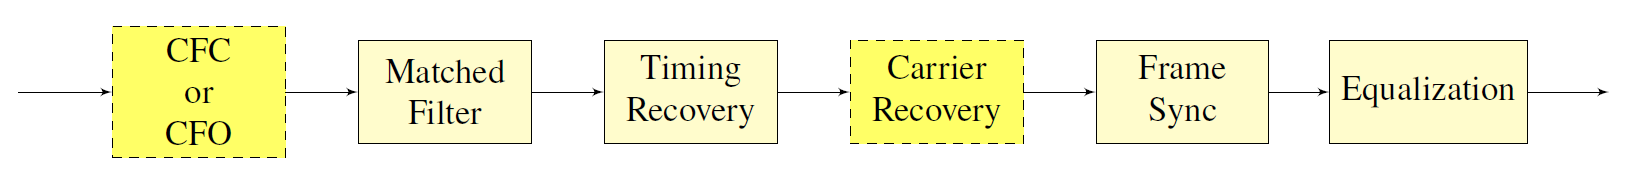
\includegraphics[width=0.8\textwidth]{receiver_block_diagram.png}}}
	\caption{Receiver Block Diagram}
	\label{fig::receiver_block_diagram}
\end{figure}

\subsection{System and Error Models}

In this experiment, we analyze a model of the receiver included in \texttt{lab6part1.m}. In this script, we model the addition of a carrier offset, $f_o$, as follows:

\begin{equation}
	r(k) = s(k)e^{j(2{\pi}f_okT+\theta)}+n(k) = s(k)e^{j(\omega_okT+\theta)}+n(k)
\end{equation}

\noindent The model generates power spectral density (PSDs) of the signal before and after the carrier offset.

Using the model, we specifically examine the effects of changing the `filterUpsample` variable, which sets the "analog" model rate, to 1. Next, with the original value of `filterUpsample`, we increase the frequency offset in unit steps of $0.1F_s$ from $0.1F_s$ to $1.0F_s$ and explain any observed effects. Then, we examine the code in \texttt{lab6part1.m} and state the reasoning behind incrementing the time vector when applying a frequency offset. Finally, we identify sources of the frequency offset besides LO mismatches.

\subsection{Coarse Frequency Correction}

In this experiment, we use a non-data aided (NDA) FFT-based technique for coarse frequency compensation. In this algorithm, we remove the PSK modulation from our received data by raising it to a power equal to modulation order. If we take an FFT of this data, the peak FFT bin should give us the frequency offset multiplied by the modulation order. For BPSK, specifically, we can estimate the frequency offset as follows:

\begin{equation}
	\label{eq::bpsk_coarse_freq_est}	
	\hat{f}_0 = \frac{1}{2TK}\underset{f}{\text{argmax}}\left\vert\sum_{k=0}^{K-1}{r^2(k)e^{-j2{\pi}kT/K}}\right\vert
\end{equation}

\noindent where $K$ is the FFT size and $T$ is the sampling period.

Using Equation \ref{eq::bpsk_coarse_freq_est} as reference, we implement a coarse frequency correction function in MATLAB using the \texttt{fft} function. To test our function, we use signals generated by \texttt{lab6part1.m}. Then, we modify Equation \ref{eq::bpsk_coarse_freq_est} to handle a QPSK signal instead of a DBPSK signal and created a function which implements the required logic.

\subsection{Fine Frequency Correction}

In this experiment, we perform fine frequency compensation. The block we implement is designed to compensate for any residual phase or frequency offsets remaining after coarse frequency compensation. The algorithm we implemented is specifically illustrated in Figure \ref{fig::fine_freq_comp_block_diagram}.

\begin{figure}[H]
	\centerline{\fbox{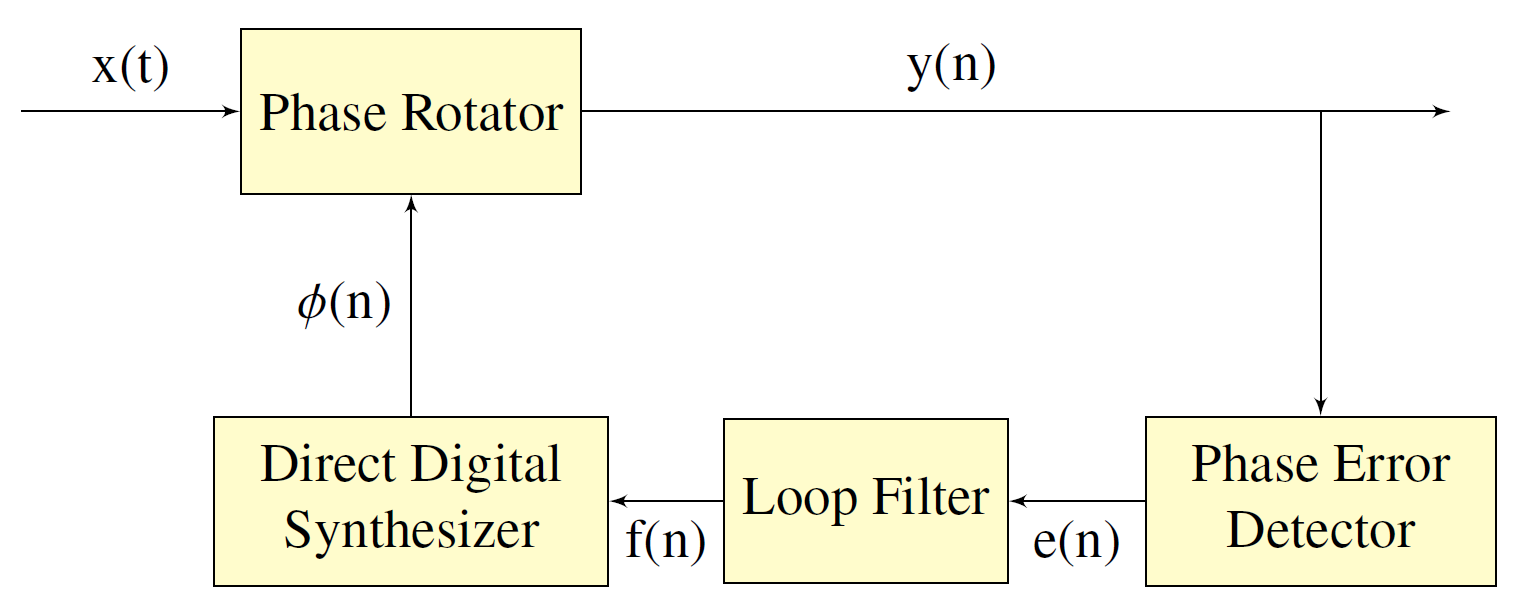
\includegraphics[width=0.6\textwidth]{fine_freq_comp_block_diagram.png}}}
	\caption{Fine Frequency Compensation}
	\label{fig::fine_freq_comp_block_diagram}
\end{figure}

In the block diagram, the phase error detector (PED) measures the phase offset of the receive samples. The loop filter governs the dynamics of the PLL. It sets the operational frequency range, lock time, and dampness/responsiveness of the PLL. Finally, the direct digital synthesizer (DDS) generates the correction signal.

The error signal output by the PED is dependent on the modulation scheme. For DBPSK modulation, it is specifically given by:

\begin{equation}
e(k) = \text{sign}(\text{Re}(y(k))) \times \text{Im}(y(k))
\end{equation}

\noindent The loop filter is a proportional-plus-integrator (PI) filter of the following form:

\begin{equation}
F(z) = G_1 + \frac{G_2}{1-z^{-1}}
\end{equation}

\noindent The gain values $G_1$ and $G_2$ are chosen based on a damping factor $\zeta$ and a loop bandwidth $B_\text{Loop}$:

\begin{align}
	\theta = \frac{B_{\text{Loop}}}{M(\zeta + 0.25/\zeta)} && \Delta = 1 + 2\zeta\theta + \theta^2
\end{align}

\begin{align}
	G_1 = \frac{4\zeta\theta/\Delta}{M} && G_2 = \frac{(4/M)\theta^2/\Delta}{M}
\end{align}

\noindent where $M$ is the constellation order. The selection of $\zeta$ affects the responsive and stability of the PLL:

\begin{equation}
\zeta = \begin{cases}
< 1, & \text{Underdamped}\\
= 1, & \text{Critically Damped}\\
> 1, & \text{Overdamped}
\end{cases}
\end{equation}

\noindent $B_\text{Loop}$ is then chosen to achieve a maximum frequency pull-in range, $\Delta_{f,\text{pull}}$, and a maximum frequency lock delay, $t_{\Delta,\text{Max}}$.

%\begin{equation}
%	\Delta_{f,\text{lock}} = \frac{4(2\pi\sqrt{2}\zeta{B_\text{Loop}})^2}{B_\text{Loop}^3}
%\end{equation}

\begin{equation}
	\Delta_{f,\text{pull}} \sim 2\pi\sqrt{2}\zeta{B_\text{Loop}}\end{equation}

\begin{equation}
	t_{\Delta,\text{Max}} \sim \frac{32\zeta^2}{B_\text{Loop}}\end{equation}
	
Using the provided equations as template, we implement fine frequency compensation (FFC) in MATLAB. We use data from \texttt{lab6part2.m} to validate our design. Next, we evaluate how the convergence times for our function are affected by different damping factors $\zeta$ and loop bandwidths $B_\text{Loop}$. Then, we compare the phase-corrected constellation to the ideal constellation using an error vector magnitude (EVM) metric, which can be computed as follows:

\begin{equation}
	\text{EVM}_\text{RMS} = 100 \times \sqrt{\frac{\frac{1}{N}\sum_{k=0}^{N-1}{e_\text{const}(k)}}{\frac{1}{N}\sum_{k=0}^{N-1}{(\text{Re}(y(k))^2 + \text{Im}(y(k))^2)}}}
\end{equation}

\noindent with

\begin{equation}
	e_\text{const}(k) = (\text{Re}(y(k)) - \text{Re}(\tilde{y}(k))^2 + (\text{Im}(y(k)) - \text{Im}(\tilde{y}(k)))^2
\end{equation}

\noindent and $\tilde{y}(k)$ defined as the reference symbol for $y(k)$. Note that we also can express the EVM in decibels as follows:

\begin{equation}
	\text{EVM}_\text{dB} = 20\text{log}_{10}(\text{EVM}_\text{RMS}/100)
\end{equation}

\noindent Finally, once we complete our EVM measurements, we figure out how the PED would have to change to support QPSK modulation.

\section{Results}
% Results and discussion of the laboratory experiment, including captured outputs, observations, and responses to laboratory questions.

\subsection{System and Error Models}

In discrete time, when we multiply a signal by a complex exponential, it circular shifts the frequency response. If we have enough excess bandwidth, we can ensure that the significant portions of our frequency response do not wrap and in turn correctly model an analog frequency shift. If we change the `filterUpsample' in \texttt{lab6part1.m} to 1, we do have any excess bandwidth. The spectrum after a frequency shift of $0.1F_s$ is shown in Figure \ref{fig::psd_upsample_1}.

\begin{figure}[H]
	\centerline{\fbox{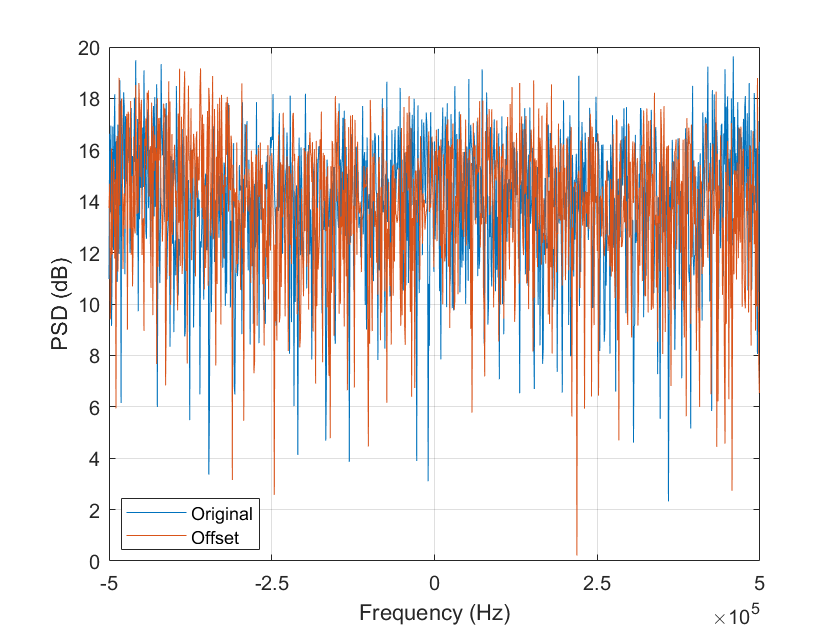
\includegraphics[width=0.5\textwidth]{psd_upsample_1.png}}}
	\caption{Frequency Response with `filterUpsample' Set to 1 and a $\protect{0.1F_s}$ Frequency Shift}
	\label{fig::psd_upsample_1}
\end{figure}

\noindent Examining the frequency response, we see that it does not correctly model a $0.1F_s$ analog frequency shift, which would have resulted in part of the spectrum being zero. Note that our updated frequency response is also not exactly a shift of the original DFT samples. This is because the DFT is sampling the DTFT. With a frequency shift of $0.1F_s$, our updated sampling positions do not overlap with the original sampling positions, which results in a slightly different response. If we instead chose a frequency shift of $F_s/16$, our sampling positions align and our DFT's are related by a simple shift. These results are captured in Figure \ref{fig::psd_upsample_1_mod_shift}.

\begin{figure}[H]
	\centerline{\fbox{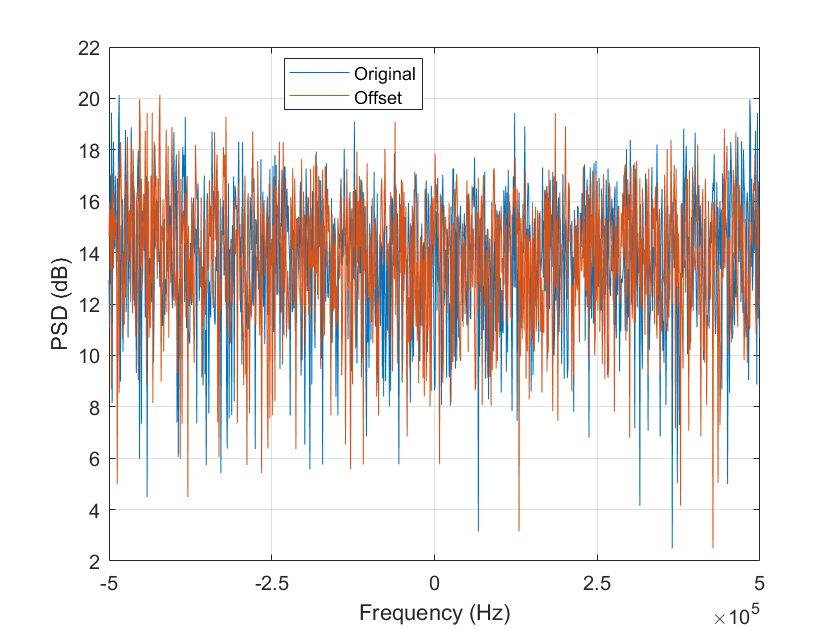
\includegraphics[width=0.5\textwidth]{psd_upsample_1_mod_shift.png}}}
	\caption{Frequency Response with `filterUpsample' Set to 1 and a $\protect{F_s/16}$ Frequency Shift}
	\label{fig::psd_upsample_1_mod_shift}
\end{figure}

\noindent We also observe a similar effect when we step the frequency offset in steps of $0.1F_s$ from $0.1F_s$ to $1.0F_s$. As we increase the frequency offset, we see the frequency response wraps. In Figure \ref{fig::psd_freq_offset_05}, we specifically show the frequency response with a frequency offset of $0.5F_s$. 

\begin{figure}[H]
	\centerline{\fbox{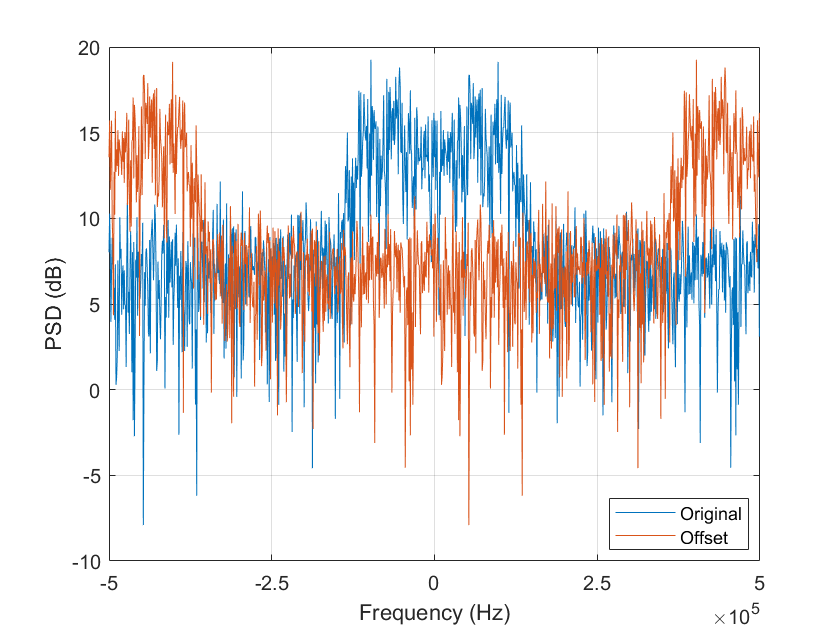
\includegraphics[width=0.5\textwidth]{psd_freq_offset_05.png}}}
	\caption{Frequency Response with a $\protect{0.5F_s}$ Frequency Shift}
	\label{fig::psd_freq_offset_05}
\end{figure}

\noindent At this frequency offset, we see that the frequency response is circularly shifted by half the bandwidth of the signal. We can explain this with DTFT properties. However, we can equivalently treat this case as an analog frequency shift prior to decimation. This results in aliasing, which in turns causes our frequency response to wrap.

	In simulation, we also increment the timing vector for each frame (\texttt{timeIndex = (k:k+frameSize-1).'}). This models back-to-back frames being fed into a continuous oscillator. The frequency offsets we observe are primarily caused by LO mismatches. However, another cause of the frequency offset is a doppler shift (which is caused by relative motion of the receiver with respect to the transmitter).

\subsection{Coarse Frequency Correction}

In this section, we perform coarse frequency correction using an FFT. To remove the modulation from our constellation, we raise our received data up to a power equivalent to the modulation order. The maximum FFT bin then gives us an index that is proportional to our estimated carrier offset. For DBPSK, the estimated carrier offset is specifically given by

\begin{equation}
	\hat{f}_0 = \frac{1}{2TK}\underset{f}{\text{argmax}}\left\vert\sum_{k=0}^{K-1}{r^2(k)e^{-j2{\pi}kT/K}}\right\vert
\end{equation}
	
\noindent When we apply coarse frequency compensation to a DBPSK-modulated signal with a $0.1F_s$ frequency offset, we obtain the spectrum shown in Figure \ref{fig::psd_bpsk_with_cfc}.

\begin{figure}[H]
	\centerline{\fbox{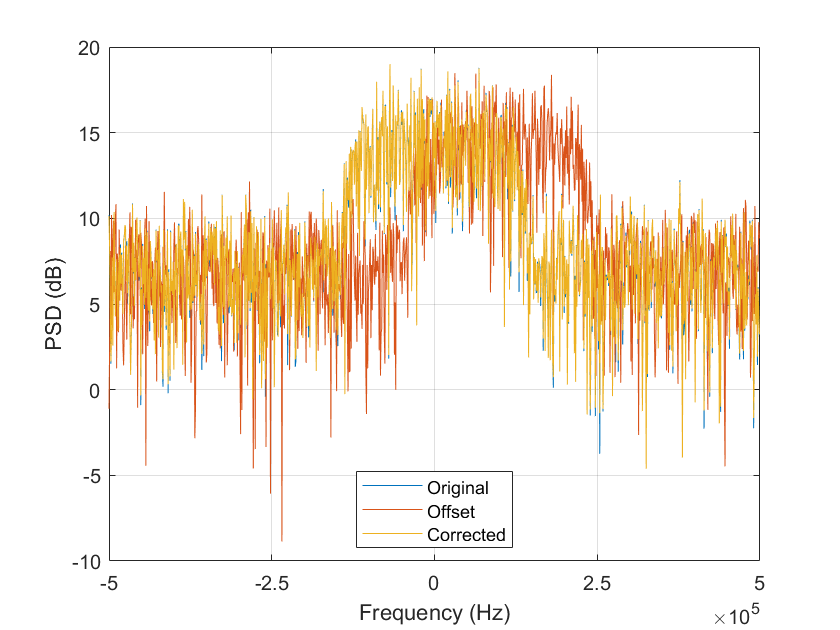
\includegraphics[width=0.5\textwidth]{psd_bpsk_with_cfc.png}}}
	\caption{DBPSK Frequency Response Before and After Coarse Frequency Correction}
	\label{fig::psd_bpsk_with_cfc}
\end{figure}

\noindent Examining the figure, we see that coarse frequency correction effectively removes the carrier offset. Our spectrum before and after compensation is essentially the same. Next, we modify our frequency offset calculation to support QPSK instead of BPSK. The resulting equation is included below:

\begin{equation}
	\hat{f}_0 = \frac{1}{4TK}\underset{f}{\text{argmax}}\left\vert\sum_{k=0}^{K-1}{r^4(k)e^{-j2{\pi}kT/K}}\right\vert
\end{equation}

\noindent Compared to our original equation, we raise our constellation points up to the 4th power instead of the 2nd power to remove the modulation. Next, we we compute our frequency offset, we have to scale the result by 1/4 instead of 1/2 to account for raising our received data to the 4th power instead of the 2nd power. When we apply coarse frequency compensation to a QPSK-modulated signal with a $0.1F_s$ frequency offset, we obtain the spectrum shown in Figure \ref{fig::psd_qpsk_with_cfc}.
 
\begin{figure}[H]
	\centerline{\fbox{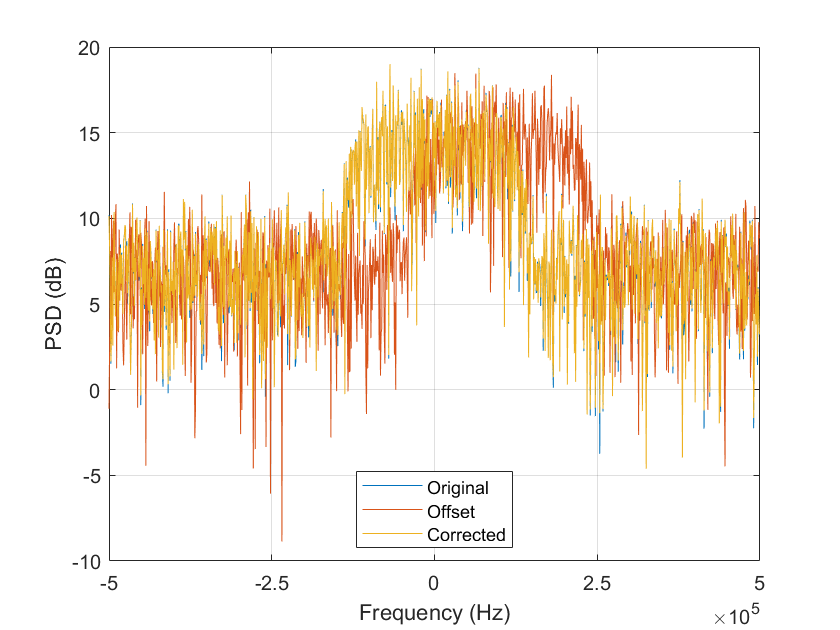
\includegraphics[width=0.5\textwidth]{psd_bpsk_with_cfc.png}}}
	\caption{QPSK Frequency Response Before and After Coarse Frequency Correction}
	\label{fig::psd_qpsk_with_cfc}
\end{figure}

\noindent Examining the resulting figure, we see that our updated equation correctly compensates for a coarse frequency offset in QPSK-modulated data.

\subsection{Fine Frequency Correction}

In this experiment, we perform fine frequency correction on a DPBPSK signal with a 20Hz frequency offset. With $B_\text{loop} = 0.01$ and $\zeta = 1/\sqrt{2}$, our constellation before and after correction is shown in Figure \ref{fig::fine_freq_comp_bpsk_const}.

\begin{figure}[H]
	\centerline{\fbox{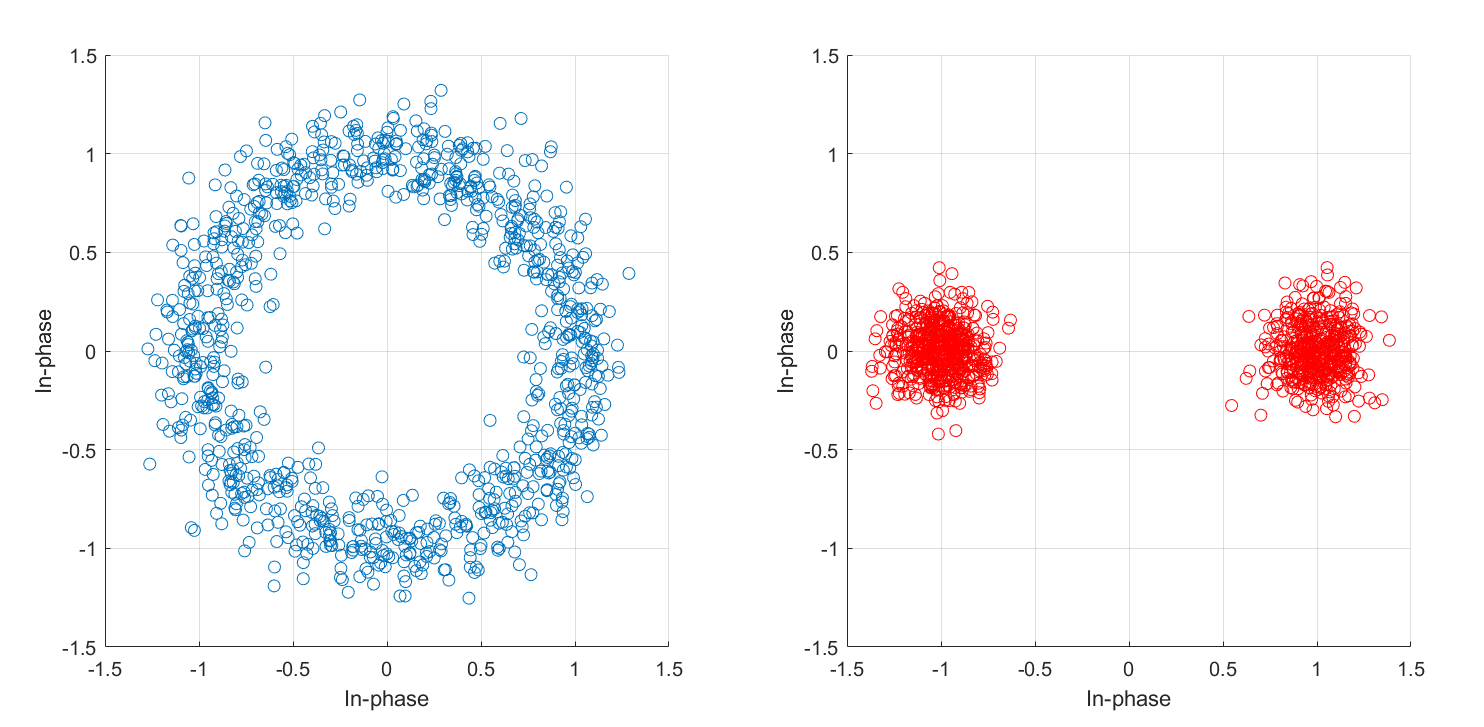
\includegraphics[width=0.8\textwidth]{fine_freq_comp_bpsk_const.png}}}
	\caption{DBPSK Constellation Before and After Fine Frequency Compensation}
	\label{fig::fine_freq_comp_bpsk_const}
\end{figure}

\noindent Qualitatively examining the figure, we see that the frequency offset has been effectively removed. We can examine the error vector magnitude to assess our error before and after compensation. 

\begin{figure}[H]
	\centerline{\fbox{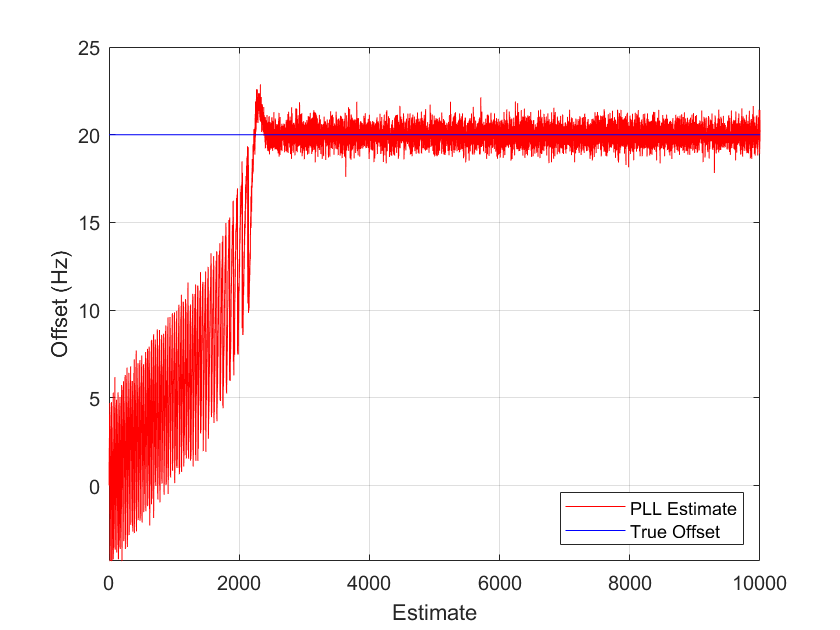
\includegraphics[width=0.5\textwidth]{convergence_Bloop_0p01_damp_sqrt_2.png}}}
	\caption{Plot of PLL Estimate for $\protect{B_\text{loop}} = 0.01$ and $\protect{\zeta = 1/\sqrt{2}}$}
	\label{fig::convergence_Bloop_0p01_damp_sqrt_2}
\end{figure}

\begin{figure}[H]
	\centerline{\fbox{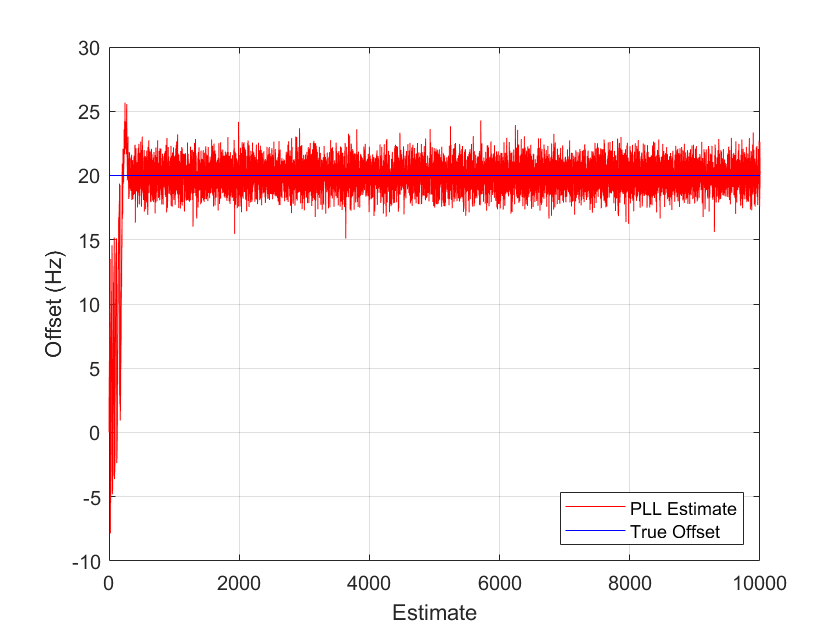
\includegraphics[width=0.5\textwidth]{convergence_Bloop_0p02_damp_sqrt_2.png}}}
	\caption{Plot of PLL Estimate for $\protect{B_\text{loop}} = 0.02$ and $\protect{\zeta = 1/\sqrt{2}}$}
	\label{fig::convergence_Bloop_0p02_damp_sqrt_2}
\end{figure}

\begin{figure}[H]
	\centerline{\fbox{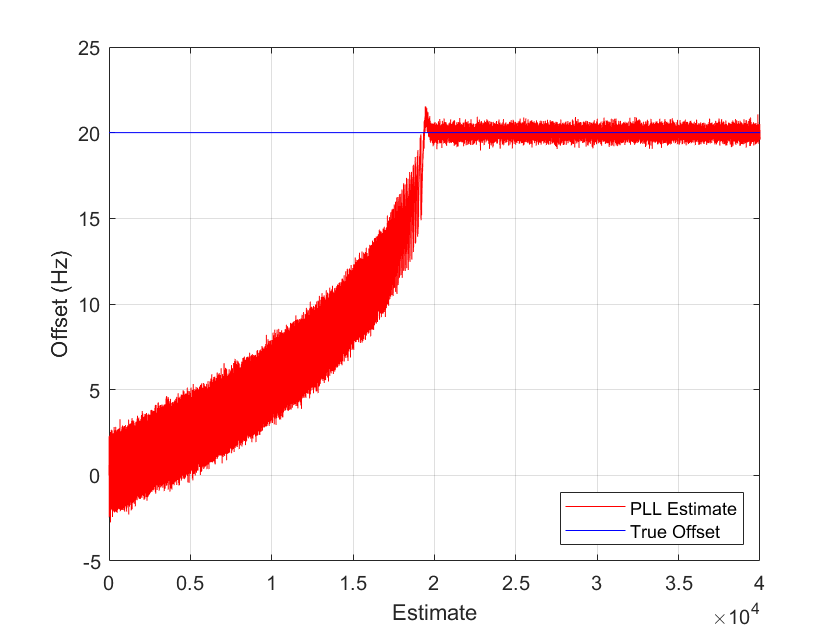
\includegraphics[width=0.5\textwidth]{convergence_Bloop_0p005_damp_sqrt_2.png}}}
	\caption{Plot of PLL Estimate for $\protect{B_\text{loop}} = 0.005$ and $\protect{\zeta = 1/\sqrt{2}}$}
	\label{fig::convergence_Bloop_0p005_damp_sqrt_2}
\end{figure}

\begin{figure}[H]
	\centerline{\fbox{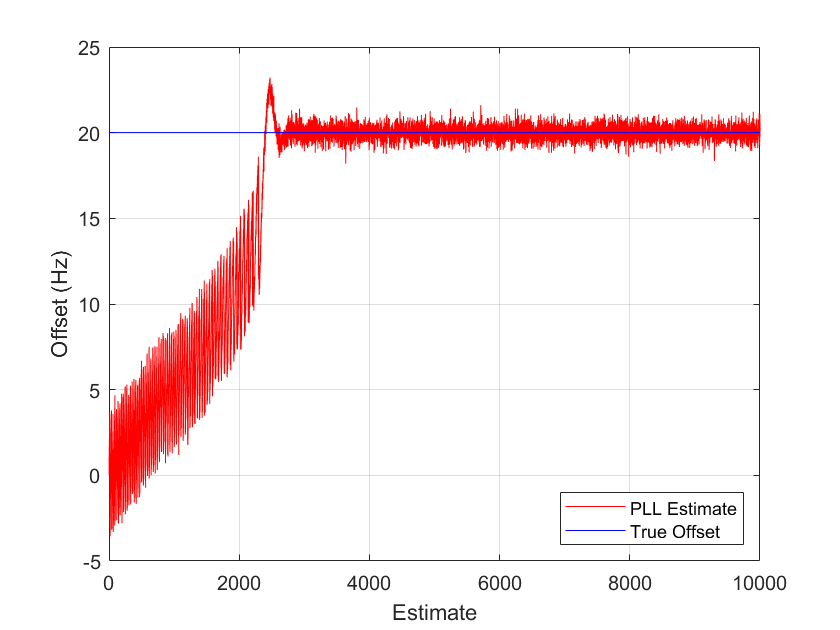
\includegraphics[width=0.5\textwidth]{convergence_Bloop_0p01_damp_0p5.png}}}
	\caption{Plot of PLL Estimate for $\protect{B_\text{loop}} = 0.01$ and $\protect{\zeta = 0.5}$}
	\label{fig::convergence_Bloop_0p01_damp_0p5}
\end{figure}

\begin{figure}[H]
	\centerline{\fbox{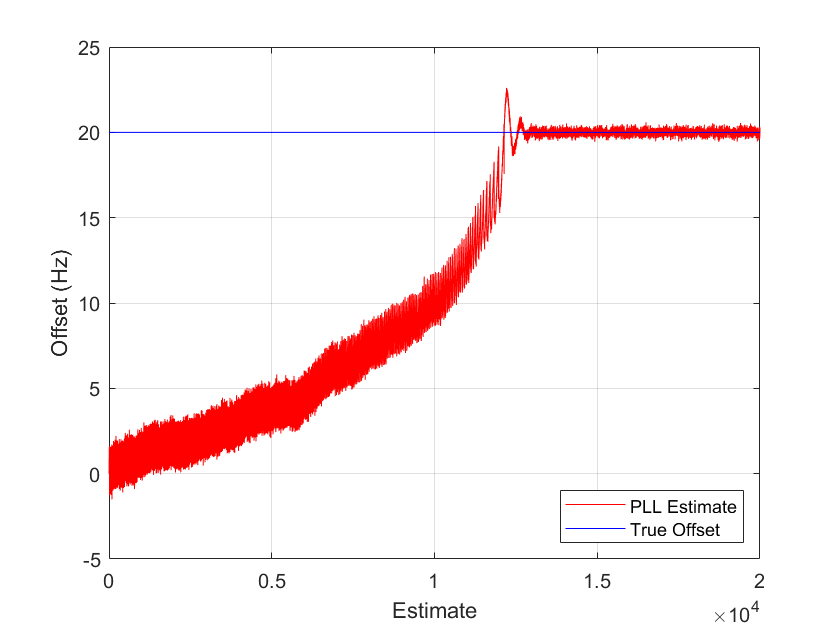
\includegraphics[width=0.5\textwidth]{convergence_Bloop_0p01_damp_0p25.png}}}
	\caption{Plot of PLL Estimate for $\protect{B_\text{loop}} = 0.01$ and $\protect{\zeta = 0.25}$}
	\label{fig::convergence_Bloop_0p01_damp_0p25}
\end{figure}

\begin{figure}[H]
	\centerline{\fbox{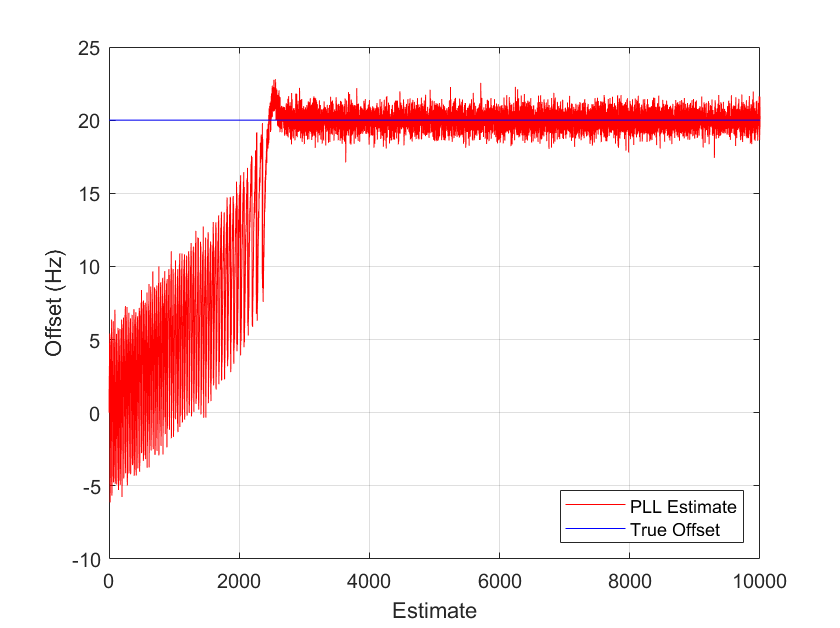
\includegraphics[width=0.5\textwidth]{convergence_Bloop_0p01_damp_1.png}}}
	\caption{Plot of PLL Estimate for $\protect{B_\text{loop}} = 0.01$ and $\protect{\zeta = 1}$}
	\label{fig::convergence_Bloop_0p01_damp_1}
\end{figure}

\begin{figure}[H]
	\centerline{\fbox{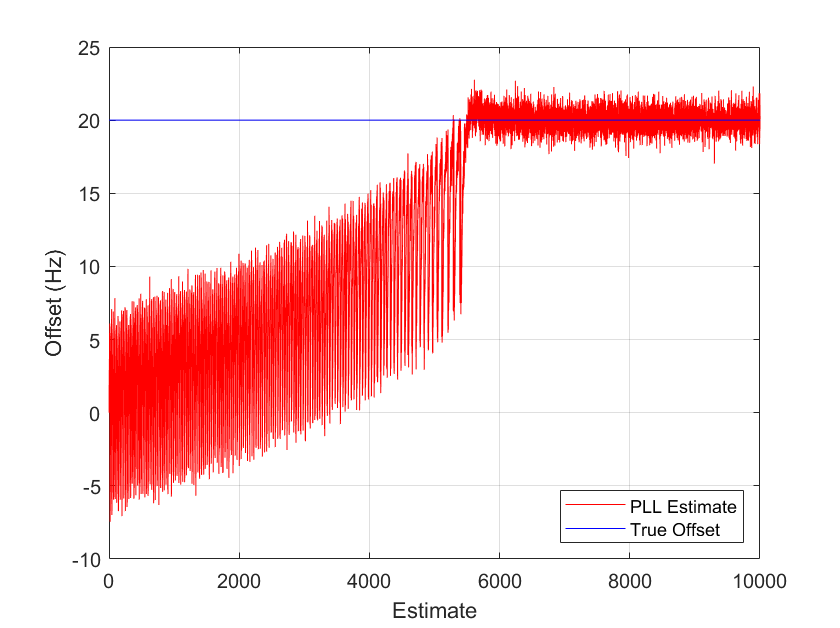
\includegraphics[width=0.5\textwidth]{convergence_Bloop_0p01_damp_2.png}}}
	\caption{Plot of PLL Estimate for $\protect{B_\text{loop}} = 0.01$ and $\protect{\zeta = 2}$}
	\label{fig::convergence_Bloop_0p01_damp_2}
\end{figure}

\noindent The QPSK PED is slightly different than the BPSK PED and is given as follows:

\begin{equation}
	\text{sign}(\text{Re}(y(n))) \times \text{Im}(y(n)) - \text{sign}(\text{Im}(y(n))) \times \text{Re}(y(n))
\end{equation}

\section{Conclusion}
% Conclusions to the overall lab that discuss meaningful lessons learned and other takeaways from the assignment. (Important)

\end{document}